%%% -*- coding: utf-8 -*-
\newpage

\chapter{Sensitive Content Dataset}
\label{chap:dataset}

In this Chapter, we present how our \textit{dataset} was collected, how it is structured, how the features were extracted, and what metrics we recommend for the main task of this dataset.

\section{Dataset Collection and Assembly}\label{sec:dataset-collection}

% falar do balanceamento e do sampling do conjunto de teste
% Falar das talbeas no texto
% colocar o resto das tabelas talvez no appendix
% estatisticas depois de dropar os maiores e os menores videos, sem balanceamento
% usamos o balanceamento dropando apesa porn videos pq os gore sao poucos
% iremos distribuir o dataset na versao balanceada e sem balanceamento
% Comparar nossas escolhas de corte de tempo com o do yt 
% Checked for duplicates by name and size and by fdupes, sem garantias de de não ter subvideos


% Before clipping video based on duration
% Mean:  0:06:18.929511  STD:  0:12:18.237458
% There are 1355 (1.05%) videos longer than 00:30:56
% There are 116 (0.09%) videos shorter than 00:00:05

\subsection{Safe content}\label{subsec:dataset-safe}

For \textit{safe content}, we chose to sample instances from Youtube8M\footnote{\url{https://research.google.com/youtube8m}}~\cite{abu2016youtube}. We chose this dataset because of the size of the dataset (8 million videos) and because of the wide variety of video classification challenges it supports. We selected 55.000 random videos inside each of the 24 top-level categories, proportionally to the original dataset distribution. As there was no limit for the sample size, we did not had to use any rules to keep small categories. 

We successfully collected 50,988 Youtube videos with metadata. 4,012 of the 55,000 sampled videos failed to download or were unavailable. 

We also collected 8,663 videos from Youtube, hereby refered as ``cherry-picked" safe videos, those videos were selected for the purpose of incremeting the amount of ``hard" videos, as done in \cite{2kdataset}, which are videos that could possibly be misclassified as sensitive, such as MMA, breastfeeding, pool party, beach and other videos that have a higher amount of skin exposure. The amount of cherry-picked videos collected are listed by its respective query in Table \ref{tab:non-yt-count}. The collection was made by automated means, an script automatically searched and tried to download all videos from the first 100 result pages of each query.

\subsection{Sensitive content}\label{subsec:dataset-sensitive}

For \textit{sensitive content}, we collected pornography and violent videography (thereafter referred to as \textit{gore}) from websites. 

For the pornography, we to sample videos from the XVideos\footnote{\url{https://info.xvideos.com/db}} database. We chose this source because of the database size (7 million videos) and because of the amount and variety of annotations. In this database, each video has one main tag, totalling 60 main tags, and tags (user-created). 

We sampled 55.000 random videos in each tag in equal proportion to the original distribution in these tags. In particular, to prevent tags with fewer videos from disappearing, we have defined that the minimum sample for each tag is the size of the smallest tag. The smallest tag was 'asmr' with 63 videos.

We successfully collected 54,549 pornography videos with metadata. 451 of the 55,000 sampled videos failed to download or were unavailable. 

We also collected 10,519 ``hard" videos from XVideos, specifically videos that have low skin exposure, fully dressed people, latex costumes, and cosplay. %8572 of those got successsfully mapped to the xvideos database and have metadata

For the gore content, we used a web crawler to extract 2,356 gore videos from various websites dedicated to gore media, such as, BestGore\footnote{\url{https://www.bestgore.com/}} and GoreBrasil\footnote{\url{https://www.gorebrasil.com}}. As these videos were the harder to find and collect, we collected all available videos from each website, no sampling method was applied. Most videos did not stay online more than one week. As there was no contact with the videos and the videos did not have any tags, all metadata collected were the title of the videos. 

Not all video's features were successfully extracted for multiple reasons, such as, corrupt data, unkown format, and missing audio. For those videos with missing audio or image, the features were still generated, but their respective modal feature were zeros. Those videos which do not had any features successfully extracted were removed from the dataset.

We also removed any duplicated videos that were detected, for duplicate video detection we used, we matched either id, title or checksum. 

\section{Dataset Structure}\label{sec:dataset-structure}

Our \textit{dataset} is structured into two main classes (or macro-classes): ``safe'' videos and sensitive videos. The sensitive macro-class is composed of two micro-classes: Pornography and Gore. The safe class is composed of videos videos from Youtube. Finally, each of the micro-classes has main-tags, which are the same main tags from their original metadata in the website, if available. Each instance (a video) of the dataset may also have tags, which are a list of tags that represent the video. The general structure and organization of our dataset is represented in Figure \ref{fig:dataset-structure}.

\begin{figure}[!ht]
    \centering
    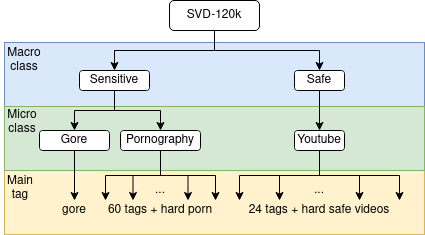
\includegraphics[width=0.95\textwidth]{img/dataset/Dataset-Structure-color.png}
    \caption{Dataset tree structure}
    \label{fig:dataset-structure}
\end{figure}


% Videos:
% Total dataset: 127075
% Total size of videos (calculated individually): 3.5TiB
% Total duration of videos (calculated indiviadually): 11806:21:13
% Improper videos: 67424
% Total size of videos (calculated individually): 1.2TiB
% Total duration of videos (calculated indiviadually): 6953:27:41
% Proper videos: 59651
% Total size of videos (calculated individually): 2.2TiB
% Total duration of videos (calculated indiviadually): 4852:53:31
% Total size of features: '896.3GiB'

There are 59,651 safe videos and 67,424 videos with sensitive content. Table \ref{tab:general-stats} presents the general statistics of our dataset, such as total duration (hours, minutes and seconds) of all videos, total (uncompressed) features size, tag coverage (If a video has at least one tag, videos may also have tags but no main tag). If played in real time, a person would take approximately 1 year and 127 days straight to flag all videos in this dataset.

\begin{table}
\centering
\caption{General statistics of the two main classes of the dataset.}
\begin{tabular}{c|r|r} 
\multicolumn{1}{l|}{} & Sensitive  & Safe        \\ 
\hline
Video Count           & 67424      & 59651       \\ 
\hline
Total Duration        & 6953:27:41 & 4852:53:31  \\ 
\hline
Mean Duration         & 00:06:11   & 00:04:52    \\ 
\hline
STD Duration          & 00:04:12   & 00:03:26    \\ 
\hline
Max Duration          & 00:30:55   & 00:30:55    \\ 
\hline
Min Duration          & 00:00:05   & 00:00:05    \\ 
\hline
Total Size            & 1.2TiB     & 2.2TiB      \\ 
\hline
Mean Size             & 19.3MiB    & 39.0MiB     \\ 
\hline
STD Size              & 35.4MiB    & 42.3MiB     \\ 
\hline
Features Size         & 519.4GiB   & 376.8GiB    \\ 
\hline
Tag coverage          & 63036      & 59651       \\ 
\hline
Tag coverage (\%)     & 93,4919    & 100,0000     \\
\end{tabular}
\label{tab:general-stats}
\end{table}

%Youtube
The Youtube micro-class has 25 main tags, as presented in Table \ref{tab:yt-granular}, in Appendix \ref{chap:appendix}, each of the videos in the "hard safe videos" main tag, has one tag, which was the query word used to collect it.

%Porn
The Pornography micro-class has 60 main tags, as presented in \ref{tab:porn-granular}, Appendix \ref{chap:appendix}, these main tags were defined by the database creators, the tags were user created. The instances in this micro-class also have user-created titles.
% Gore
There are no main-tags or tags (but the 'gore' tag) on the Gore micro-class as they were not available on their site. All instances, however, have user-created titles.

\begin{table}
\centering
\caption{Granular statistics of the dataset: Videos collected from Youtube, pornographic videos, and gore videos.}
\begin{tabular}{c|r|r|r} 
\multicolumn{1}{l|}{} & \multicolumn{1}{c|}{Pornography} & \multicolumn{1}{c|}{Gore} & \multicolumn{1}{c}{YouTube}  \\ 
\hline
Video Count           & 65068                     & 2356                      & 59651                         \\ 
\hline
Total Duration        & 6900:17:38                & 53:10:02                  & 4852:53:31                    \\ 
\hline
Mean Duration         & 00:06:21                  & 00:01:21                  & 00:04:52                      \\ 
\hline
STD Duration          & 00:04:10                  & 00:01:26                  & 00:03:26                      \\ 
\hline
Max Duration          & 00:30:55                  & 00:16:56                  & 00:30:55                      \\ 
\hline
Min Duration          & 00:00:05                  & 00:00:05                  & 00:00:05                      \\ 
\hline
Total Size            & 1.2TiB                    & 15.8GiB                   & 2.2TiB                        \\ 
\hline
Mean Size             & 19.8MiB                   & 6.9MiB                    & 39.0MiB                       \\ 
\hline
STD Size              & 35.9MiB                   & 13.9MiB                   & 42.3MiB                       \\ 
\hline
Features Size         & 515.3GiB                  & 4.1GiB                    & 376.8GiB                      \\ 
\hline
Tag coverage          & 63036                     & 0                      & 59651                         \\ 
\hline
Tag coverage (\%)     & 96,8771                   & 0                  & 100,0000                       \\
\end{tabular}
\label{tab:granular-stats}
\end{table}

By using macro and micro classes of this dataset, our dataset  also supports other tasks, other than binary classification of sensitive content, such as:
\begin{itemize}
    \item Multi label classification (or tagging) of pornographic videos;
    \item Multi label classification of "Safe" (Videos that do not contain sensitive content);
    \item Binary classification of extremely violent videos;
    \item Binary classification of pornography.
\end{itemize}


\subsection{Dataset Distribution}\label{sec:distribution}

The dataset will be distributed as extracted and processed visual and audio features from the videos. Each instance (features from a video) is associated with a id, a label, and a sequence size. General details on the dataset distribution are available in Appendix \ref{chap:datasheet}.



\subsection{Dataset Balancing}\label{sec:balancing}

For experimenting, we equally balanced both main labels (sensitive/improper and safe/proper), so that both main classes have the same number of instances. One could also choose not to balance both classes equally, since our main metric already take label imbalance into account.
Additionally, when removing excess sensitive content (while balancing), we removed only pornography videos in order to not lower the amount of gore videos.


\subsection{Dataset splits and Test sets}\label{sec:testsets}

We hold out our dataset for testing  our approach: 10\% of the safe videos, then 10\% of gore videos, and sample a number of pornography to to match the amount of safe videos minus the amount of gore test samples, so that the test subset has a balanced amount of sensitive and safe videos, while keeping a valid amount of gore videos. For the micro-classes that have multiple main tags (Youtube and Pornography), we took stratified samples based on the number of each main tag in the dataset. The number of instance by micro-class sampled is presented in Table \ref{tab:subset-stats}.

\begin{table}
\centering
\caption{Test subset statistics.}
\begin{tabular}{l|l|l|l}
                  & Pornography & Gore     & YouTube   \\ \hline
Video Count       & 5732        & 236      & 5968      \\ \hline
Total Duration    & 574:03:29   & 05:22:20 & 443:35:36 \\ \hline
Mean Duration     & 00:06:00    & 00:01:21 & 00:04:27  \\ \hline
STD Duration      & 00:03:44    & 00:01:48 & 00:02:32  \\ \hline
Max Duration      & 00:30:29    & 00:16:56 & 00:29:01  \\ \hline
Min Duration      & 00:00:05    & 00:00:07 & 00:00:07  \\ \hline
Total Size        & 80.2GiB     & 1.5GiB   & 204.8GiB  \\ \hline
Mean Size         & 14.3MiB     & 6.6MiB   & 35.1MiB   \\ \hline
STD Size          & 25.6MiB     & 14.4MiB  & 35.0MiB   \\ \hline
Features Size     & 42.6GiB     & 424.1MiB & 34.5GiB   \\ \hline
Tag coverage      & 5695        & 0        & 5968      \\ \hline
Tag coverage (\%) & 99,3545     & 0,0000   & 100,0000 
\end{tabular}
\label{tab:subset-stats}
\end{table}

As a complementary test dataset, we selected the NPDI 2k-pornography dataset~\cite{avila2013pooling}, it contains 1000 non-pornographic videos and 1000 pornographic videos. Those non-pornographic videos are comprised of ``hard'' and ``easy'' videos according to the likelihood of misclassification. Some examples of ``hard'' videos are those with high amounts of exposed skin, such as swimming and sumo fighting videos. Its general statistics are shown in Table \ref{tab:2kdataset-stats}.

\begin{table}
\centering
\caption{NPDI 2k-pornography dataset statistics.}
\begin{tabular}{c|r|r} 
\multicolumn{1}{l|}{} & \multicolumn{1}{c|}{Porn} & \multicolumn{1}{c}{Non-Porn}  \\ 
\hline
Video Count           & 1000                      & 1000                           \\ 
\hline
Total Duration        & 100:30:32                 & 40:26:06                       \\ 
\hline
Mean Duration         & 00:06:01                  & 00:02:25                       \\ 
\hline
STD Duration          & 00:05:49                  & 00:02:17                       \\ 
\hline
Max Duration          & 00:33:40                  & 00:20:16                       \\ 
\hline
Min Duration          & 00:00:05                  & 00:00:02                       \\ 
\hline
Total Size            & 26.4GiB                   & 18.5GiB                        \\ 
\hline
Mean Size             & 27.0MiB                   & 18.9MiB                        \\ 
\hline
STD Size              & 31.1MiB                   & 21.9MiB                        \\ 
\hline
Features Size         & 7.6GiB                    & 3.1GiB                         \\ 
\hline
Tag coverage          & 0                      & 0                           \\ 
\hline
Tag coverage (\%)     & 0                       & 0                            \\
\end{tabular}
\label{tab:2kdataset-stats}
\end{table}

\section{Metrics}\label{sec:metrics}

% in binary classification, recall of the positive class is also known as “sensitivity”; recall of the negative class is “specificity”.
%https://en.wikipedia.org/wiki/Sensitivity_and_specificity
%https://en.wikipedia.org/wiki/Precision_and_recall

To evaluate each experiment and our approach, we will use Precision (P), Recall (R) and, most importantly, the weighted F2-score. In this section we present a contextualized explanation these metrics.

% FROM: de morereira et al 2019
%For assessing the performance of the pornography locators, we re-port thenormalized classification accuracyrate (ACC), and theF2measure(F2). Prior to explaining ACC, we need to definerecallandspecificityfrom the point of view of pornography localization.  Specificity, in turn, measures the capacity of alocator to correctly identify truly negative video seconds as so. A spe-cificity of only 50%, for example, means the system mislabels one inevery two seconds of non-pornographic content, wrongly identifying itas sensitive. In this vein, ACC is the mean of recall and specificity. Ahigher accuracy indicates a higher capability of separating porno-graphic video seconds from non-pornographic ones.F2measure, in turn, is a more complex metric that depends also onthe concept ofprecision. From the point of view of pornography loca-lization, precision expresses how many seconds are truly relevant (i.e.,pornographic), among all the ones that a locator identifies as such.Therefore, F2is the weighted harmonic mean of recall and precision,which gives twice more weight to recall than to precision, by means of a=β2parameter.Eq. (7)depicts the original Fβformula=+ ×××+Fβprecision  recallβ   precision  recall(1    ),β22(7)in which we use=β2. In doing so, F2lets us pay more attention to therecall of the solutions, rather than to their precision. This is usefulbecause, in the case of pornographyfiltering, false-negative answers areworse than the false-positive ones. It is less prejudicial to wrongly denythe access to non-pornographic content, than to wrongly disclose por-nographic content. Hence, we can consider that a solution with higherF2measure is better, because it cares more about how many porno-graphic video seconds are really beingfiltered out (recall), instead ofhow many“supposedly”positive seconds are indeed pornographic(precision)



In the context of sensitive content detection, \textit{true positives} are videos predicted as sensitive and are in fact, sensitive. Likewise, \textit{true negatives} are videos predicted as safe and are indeed safe. \textit{False positives} are videos predicted as sensitive, but were safe, the same goes for \textit{false negatives}, which are videos that were predicted as safe, but were actually sensitive.

% from the daniel moreira paper:
% thenormalized classification accuracyrate (ACC)ACC is the mean of recall and specificity. Ahigher accuracy indicates a higher capability of separating porno-graphic video seconds from non-pornographic ones

Precision (Equation~\ref{equation:precision}) measures how many videos predicted as sensitive (both true positives and false positives) are truly sensitive. The Recall (Equation~\ref{equation:recall})  measures how many truly positive videos were correctly identified.

\begin{multicols}{2}
  \begin{equation}
    \label{equation:precision}
    P = \frac{TP}{TP + FP}
  \end{equation}

  \begin{equation}
    \label{equation:recall}
    R = \frac{TP}{TP + FN}
  \end{equation}
  
\end{multicols}

Where $TP, TN, FP$, and $FN$ denote the examples that are true positives, true negatives, false-positives, and false negatives, respectively.

\begin{equation}
\label{equation:fbeta}
F_\beta = (1+\beta^2) \times \frac{P \times R}{(\beta^2 \times P) + R}
\end{equation}

The $F_\beta$-score, defined in Equation~\ref{equation:fbeta}, evaluates the classifier by the harmonic mean between Precision and Recall. To account for label imbalance, after calculating the F2-score metrics for each label, we find their average weighted by support (the number of true instances for each label). 

Most related works use either F1-score ($\beta=1$) or F2-score ($\beta=2$) metrics as their main evaluation metric. While the F1-score represents an balanced performance metric, the F2-score gives twice more weight to the recall than to precision, which means that the metric is more focused on the recall of a solution.

% in the case of pornographyfiltering, false-negative answers areworse than the false-positive ones. It is less prejudicial to wrongly denythe access to non-pornographic content, than to wrongly disclose por-nographic content. Hence, we can consider that a solution with higherF2measure is better, because it cares more about how many porno-graphic video seconds are really beingfiltered out (recall), instead ofhow many“supposedly”positive seconds are indeed pornographic(precision)
In this work, the F2-score represents an overall performance metric, while the precision and recall metrics can give insights on what the classifier model is doing better and what to improve. We chose the weighted F2-score as our main evaluation metric because when detecting sensitive content it is more important to predict a truly sensitive video than to predict a safe video as sensitive.
